\documentclass[letterpaper,10pt]{article}

\usepackage{latexsym}
\usepackage[empty]{fullpage}
\usepackage{titlesec}
\usepackage{marvosym}
\usepackage[usenames,dvipsnames]{color}
\usepackage{verbatim}
\usepackage{enumitem}
\usepackage[hidelinks]{hyperref}
\usepackage{fancyhdr}
\usepackage[english]{babel}
\usepackage{tabularx}
\usepackage{tikz}
\usetikzlibrary{arrows.meta,calc,positioning}
\usepackage{iftex}
\ifPDFTeX
  \input{glyphtounicode}
\fi

\pagestyle{fancy}
\fancyhf{}
\fancyfoot{}
\renewcommand{\headrulewidth}{0pt}
\renewcommand{\footrulewidth}{0pt}

\addtolength{\oddsidemargin}{-0.5in}
\addtolength{\evensidemargin}{-0.5in}
\addtolength{\textwidth}{1in}
\addtolength{\topmargin}{-.75in}
\addtolength{\textheight}{1.35in}

\urlstyle{same}
\raggedbottom
\raggedright
\setlength{\tabcolsep}{0in}
\ifPDFTeX
  \pdfgentounicode=1
\fi

\titleformat{\section}{
  \vspace{-9pt}\scshape\raggedright\large
}{}{0em}{}[\color{black}\titlerule \vspace{-8pt}]

\newcommand{\resumeItem}[1]{
  \item\small{{#1 \vspace{-3pt}}}
}

\newcommand{\resumeSubheading}[4]{
  \vspace{-2pt}\item
    \begin{tabular*}{0.97\textwidth}[t]{l@{\extracolsep{\fill}}r}
      \textbf{#1} & #2 \\
      \textit{\small#3} & \textit{\small #4} \\
    \end{tabular*}\vspace{-7pt}
}

\newcommand{\resumeProjectHeading}[2]{
  \item
  \begin{tabular*}{0.97\textwidth}{l@{\extracolsep{\fill}}r}
    \small#1 & #2 \\
  \end{tabular*}\vspace{-7pt}
}

\newcommand{\resumeSubHeadingListStart}{
  \begin{itemize}[leftmargin=0.15in, label={}]
}

\newcommand{\resumeSubHeadingListEnd}{
  \end{itemize}
}

\newcommand{\resumeItemListStart}{
  \begin{itemize}[leftmargin=0.2in, topsep=0pt, itemsep=0pt]
}

\newcommand{\resumeItemListEnd}{
  \end{itemize}\vspace{-4pt}
}

\definecolor{agentedge}{HTML}{C48A3A}
\definecolor{humanedge}{HTML}{C45C5C}
\definecolor{nodefill}{HTML}{E8F0FA}
\definecolor{nodedraw}{HTML}{4A6FA5}

\tikzset{
  rbox/.style={
    draw=nodedraw,
    fill=nodefill,
    rounded corners=2pt,
    align=center,
    font=\tiny\sffamily,
    inner sep=2.4pt,
    minimum height=0.34cm,
  },
  roval/.style={
    rbox,
    circle,
    minimum size=0.98cm,
    inner sep=0.6pt,
  },
  agentarr/.style={
    -{Stealth[length=1.7mm]},
    line width=0.75pt,
    draw=agentedge,
  },
  humanarr/.style={
    -{Stealth[length=1.7mm]},
    line width=0.8pt,
    draw=humanedge,
  },
  edgelabel/.style={
    font=\tiny\sffamily,
    inner sep=1pt,
    align=center,
  },
}

\begin{document}

%----------HEADING----------

\begin{center}
  \textbf{\Huge \scshape Weishu Zhang} \\ \vspace{3pt}
  \small
  626-566-4310 $|$
  \href{mailto:weszhang@berkeley.edu}
  {\underline{weszhang@berkeley.edu}} $|$
  \href{https://linkedin.com/in/Weishuz}
  {\underline{LinkedIn}} $|$
  \href{https://github.com/WeishuZ}
  {\underline{GitHub}} $|$
  \href{https://weishuz.com/}
  {\underline{Website}}
\end{center}

\vspace{-6pt}

\begin{center}
  \small
  Backend-leaning full-stack engineer building production agent systems
  and enterprise workflow runtimes.
\end{center}

%----------EDUCATION----------

\section{Education}

\resumeSubHeadingListStart

  \resumeSubheading
    {University of California, Berkeley}{Berkeley, CA}
    {Bachelor of Science in Electrical Engineering and Computer Sciences}
    {May 2027}

    \resumeItemListStart
      \resumeItem{
        \textbf{GPA: 4.0/4.0}.
        Coursework: Efficient Algorithms, Network Science, Artificial Intelligence
      }
    \resumeItemListEnd

\resumeSubHeadingListEnd

%----------TECHNICAL SKILLS----------

\section{Technical Skills}

\begin{itemize}[leftmargin=0.15in, label={}]
  \small{
    \item{
      \textbf{Languages}{:
        Python, TypeScript/JavaScript, SQL, Java, Go, C/C++
      } \\

      \textbf{Full Stack}{:
        React, Next.js, Node.js, FastAPI, PostgreSQL, Redis, SQLite,
        REST APIs
      } \\

      \textbf{AI \& Agents}{:
        LangGraph, MCP, LLM APIs, agent runtimes, structured generation,
        PyTorch, vLLM, QLoRA
      } \\

      \textbf{Infrastructure}{:
        Temporal, durable workflows, Docker, Kubernetes, gVisor, OCI,
        OpenTelemetry, pytest, distributed jobs, CI/CD
      }
    }
  }
\end{itemize}

%----------EXPERIENCE----------

\section{Experience}

\resumeSubHeadingListStart

  \resumeSubheading
    {Amazon AI Studio}{}
    {Incoming Software Development Engineer Intern}
    {Sep 2026 -- Nov 2026}

  \vspace{5pt}

  \resumeSubheading
    {ASML}{San Jose, CA}
    {Software Engineering in Test Intern}
    {2026 -- Present}

    \resumeItemListStart

      \resumeItem{
        Designed the \textbf{runtime agent infrastructure} for Tachyon SQA:
        daily regression tracking and a durable \textbf{test-plan lifecycle}
        (draft $\rightarrow$ QA approval $\rightarrow$ async job execution
        $\rightarrow$ result writeback).
      }
      \resumeItem{
        Built a \textbf{human-governed self-evolution} loop: reusable session
        memory is staged into shared memory, audited by humans, then persisted
        into the harness.
      }
      \resumeItem{
        Implemented \textbf{Temporal-style durable execution}: deterministic
        workflows, activities, QA-approval signals, task-queue claiming,
        idempotent writes, event-history replay, and sandbox recovery.
      }
    \resumeItemListEnd

    \vspace{1pt}
    \hspace*{-0.12in}%
    \begin{minipage}[t]{0.50\textwidth}
      \centering
      \resizebox{0.98\linewidth}{!}{%
      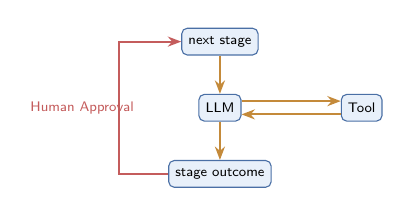
\begin{tikzpicture}
        \node[rbox] (next) at (1.05,1.70) {next stage};
        \node[rbox] (llm)  at (1.05,0.86) {LLM};
        \node[rbox] (tool) at (2.85,0.86) {Tool};
        \node[rbox] (out)  at (1.05,0.02) {stage outcome};
        \draw[agentarr] (next) -- (llm);
        \draw[agentarr] ([yshift=2.4pt]llm.east) -- ([yshift=2.4pt]tool.west);
        \draw[agentarr] ([yshift=-2.4pt]tool.west) -- ([yshift=-2.4pt]llm.east);
        \draw[agentarr] (llm) -- (out);
        \draw[humanarr] (out.west) -- ++(-0.62,0) |- (next.west);
        \node[edgelabel, anchor=east, text=humanedge] at (0.00,0.86)
          {Human Approval};
      \end{tikzpicture}}\\[1pt]
      {\tiny Human-gated stage loop}
    \end{minipage}
    \hfill
    \begin{minipage}[t]{0.48\textwidth}
      \centering
      \resizebox{0.98\linewidth}{!}{%
      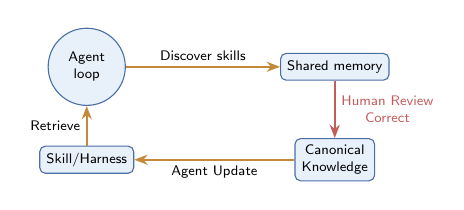
\begin{tikzpicture}
        \node[roval] (loop)   at (0.00,1.18) {Agent\\loop};
        \node[rbox]  (shared) at (3.15,1.18) {Shared memory};
        \node[rbox]  (canon)  at (3.15,0.00) {Canonical\\Knowledge};
        \node[rbox]  (skill)  at (0.00,0.00) {Skill/Harness};
        \draw[agentarr] (loop) --
          node[edgelabel, above, yshift=1pt] {Discover skills} (shared);
        \draw[humanarr] (shared) --
          node[edgelabel, right, text=humanedge, xshift=1pt]
            {Human Review\\Correct} (canon);
        \draw[agentarr] (canon) --
          node[edgelabel, below, yshift=-1pt] {Agent Update} (skill);
        \draw[agentarr] (skill) --
          node[edgelabel, left, xshift=-1pt] {Retrieve} (loop);
      \end{tikzpicture}}\\[1pt]
      {\tiny Human-governed skill evolution}
    \end{minipage}
    \vspace{1pt}
  \resumeSubheading
    {Open Ludus}{Remote}
    {Co-Founder \& Software Engineer, Cloud Agent Infrastructure}
    {2026 -- Present}

    \resumeItemListStart

      \resumeItem{
        Designed a \textbf{Kubernetes-native agent sandbox control plane} using
        CRDs and controllers to reconcile isolated, stateful workspaces from
        reusable runtime templates, with warm-pool provisioning, suspend/resume,
        and TTL-based garbage collection.
      }

      \resumeItem{
        Hardened untrusted-code execution with \textbf{gVisor/Kata
        RuntimeClasses}, namespace-scoped service accounts and RBAC,
        default-deny NetworkPolicies, restricted pod security contexts, and
        CPU, memory, and ephemeral-storage quotas.
      }

      \resumeItem{
        Standardized reproducible agent environments using immutable OCI images,
        validated configuration and short-lived secret projection, repository
        bootstrap, and PVC-backed workspaces; instrumented provisioning and
        execution with OpenTelemetry traces and lifecycle metrics.
      }

    \resumeItemListEnd

  \resumeSubheading
    {Berkeley Artificial Intelligence Research (BAIR)}
    {Berkeley, CA}
    {Undergraduate Research Assistant}
    {Jan 2026 -- Present}

    \resumeItemListStart

      \resumeItem{
        Led expert task acquisition for the
        \textbf{Agent Human Last Exam} benchmark, recruiting
        \textbf{30+ domain experts} and contributing to the collection of
        \textbf{80+} complex, cross-domain agent tasks.
      }

      \resumeItem{
        Built an LLM-powered proposal agent that converts rough expert ideas
        into structured benchmark tasks, supporting iterative refinement,
        constraint checking, and higher-quality submissions.
      }

    \resumeItemListEnd

  \resumeSubheading
    {University of California, San Francisco}
    {San Francisco, CA}
    {Software Research Assistant}
    {Aug 2025 -- Present}

    \resumeItemListStart

      \resumeItem{
        Built a production-oriented long-context clinical information
        extraction pipeline, increasing inference throughput by \textbf{3x}
        and reducing VRAM usage by approximately \textbf{80\%} using vLLM,
        paged attention, quantization, and batched execution.
      }

      \resumeItem{
        Created a \textbf{4,000+}-example domain dataset, fine-tuned Qwen
        models with QLoRA, and implemented validation and self-consistency
        checks that maintained \textbf{100\% schema-valid} structured outputs.
      }

    \resumeItemListEnd

\resumeSubHeadingListEnd

%----------OPEN SOURCE AND PROJECTS----------

\section{Open Source \& Projects}

\resumeSubHeadingListStart

  \resumeProjectHeading
    {
      \textbf{
        \href{
          https://github.com/pytorch/pytorch/pulls?q=is\%3Apr+author\%3AWeishuZ
        }{PyTorch}
      }
      $|$
      \emph{torch.compile, torch.export, Dynamo}
      \hfill
      \href{
        https://github.com/pytorch/pytorch/pulls?q=is\%3Apr+author\%3AWeishuZ
      }{\underline{PRs}}
    }
    {}

    \resumeItemListStart
      \resumeItem{
        Production fixes to \textbf{pytorch/pytorch} compiler and export
        internals: eager-versus-compiled gaps, tracing failures, and export
        regressions, with maintainer-reviewed tests.
      }
    \resumeItemListEnd

  \resumeProjectHeading
    {
      \textbf{
        \href{https://gradeview.eecs.berkeley.edu/}{GradeView}
      }
      $|$
      \emph{React, TypeScript, Python, PostgreSQL, Redis}
      \hfill
      \href{https://gradeview.eecs.berkeley.edu/}
      {\underline{Live}}
      $|$
      \href{
        https://youtu.be/n9Dsu-5s7IM?si=fq_MlZXKm52iiy5T
      }{\underline{Demo}}
      $|$
      \href{
        https://dl.acm.org/doi/10.1145/3770761.3777343
      }{\underline{Poster}}
    }
    {}

    \resumeItemListStart
      \resumeItem{
        Refactored Berkeley course analytics into containerized
        React/Node/Python services, with PostgreSQL as source of truth and
        Redis cache prewarming.
      }
    \resumeItemListEnd

\resumeSubHeadingListEnd

\end{document}
